
\documentclass[conference]{IEEEtran}
\IEEEoverridecommandlockouts
% The preceding line is only needed to identify funding in the first footnote. If that is unneeded, please comment it out.
\usepackage{cite}
\usepackage{amsmath,amssymb,amsfonts}
\usepackage{algorithmic}
\usepackage{graphicx}
\usepackage{textcomp}
\usepackage{xcolor}
\usepackage{float}
\usepackage{listings}

\usepackage{xcolor}

\definecolor{codegreen}{rgb}{0,0.6,0}
\definecolor{codegray}{rgb}{0.5,0.5,0.5}
\definecolor{codepurple}{rgb}{0.58,0,0.82}
\definecolor{backcolour}{rgb}{0.95,0.95,0.92}

\lstdefinestyle{mystyle}{
    backgroundcolor=\color{backcolour},   
    commentstyle=\color{codegreen},
    keywordstyle=\color{magenta},
    numberstyle=\tiny\color{codegray},
    stringstyle=\color{codepurple},
    basicstyle=\ttfamily\footnotesize,
    breakatwhitespace=false,         
    breaklines=true,                 
    captionpos=b,                    
    keepspaces=true,                 
    numbers=left,                    
    numbersep=5pt,                  
    showspaces=false,                
    showstringspaces=false,
    showtabs=false,                  
    tabsize=2
}

\lstset{style=mystyle}

\def\BibTeX{{\rm B\kern-.05em{\sc i\kern-.025em b}\kern-.08em
    T\kern-.1667em\lower.7ex\hbox{E}\kern-.125emX}}

\begin{document}

\makeatletter
\newcommand{\linebreakand}{%
    \end{@IEEEauthorhalign}
    \hfill\mbox{}\par
    \mbox{}\hfill\begin{@IEEEauthorhalign}
}
\makeatother

\title{Problema 2: Implementação da Conversão Analógico-Digital (AD) de n bits\\
}

\author{
    \IEEEauthorblockN{1\textsuperscript{st} João Victor Oliveira Couto}
    \IEEEauthorblockA{\textit{Estudante de Eng. de Computação} \\
        \textit{Universidade Estadual de Feira de Santana}\\
        Feira de Santana, Bahia, Brasil \\
        contact@jityvoo.dev}
    \and
    \IEEEauthorblockN{2\textsuperscript{nd} Velder Soares}
    \IEEEauthorblockA{\textit{Estudante de Eng. de Computação} \\
        \textit{Universidade Estadual de Feira de Santana}\\
        Feira de Santana, Bahia, Brasil \\
        velder.vas@gmail.com}
    \IEEEauthorblockN{}
    \IEEEauthorblockA{}
}

\maketitle

\begin{abstract}
    Este relatório aborda a análise espectral de sinais discretos usando a Transformada Discreta de Fourier no Tempo (DTFT) e sua implementação prática através da FFT. O experimento foi realizado a partir de um sinal gerado e amostrado em diferentes taxas (50 kHz, 20 kHz, 10 kHz, 5 kHz e 2 kHz) utilizando um Arduino ATMega2560. O sinal amostrado foi transferido para o ambiente Octave, onde a FFT foi aplicada para calcular o espectro e observar as componentes de frequência. Além disso, janelas foram aplicadas ao sinal para minimizar o vazamento espectral e melhorar a definição do espectro. A resolução espectral foi analisada em função do número de amostras, destacando como esse fator influencia a precisão das componentes espectrais. Os resultados mostram que, mesmo com um número reduzido de amostras, as frequências principais do sinal ainda podem ser identificadas, possibilitando a reconstrução do sinal, desde que o critério de Nyquist seja respeitado. O relatório conclui que o número de amostras e o uso de janelas são determinantes para a qualidade da análise espectral.


\end{abstract}

\begin{IEEEkeywords}
    Conversão analógico-digital, Transformada de Fourier, Transformada Discreta de Fourier no Tempo
\end{IEEEkeywords}

\section{Introdução}
Em termos físicos e naturais, as grandezas variam de forma contínua e analógica, onde cada instante de tempo infinitesimal pode apresentar um valor que varie. Hoje, sistemas automatizados coletam dados externos analógicos, como pressão em reservatórios, temperatura em caldeiras, sinais de áudio, dentre outros.

Por outro lado, os sistemas digitais operam com sinais quantizados. Isso significa que, para processar informações analógicas, é frequentemente necessário convertê-las em um formato compatível com o processamento digital. Para esse propósito, são empregados conversores analógico-digitais (também conhecidos como A/D ou ADC), cuja compreensão das características e funcionalidades é essencial.

Portanto, entender as características dos conversores A/D e como os mesmos funcionam, se torna fundamental. Neste trabalho, iremos nos concentrar na análise da função e características dos conversores A/D de Rampa Dupla.


\section{Desenvolvimento}
% Aqui entra a pasta com o conteúdo de como a análise analítica foi realizada
Um conversor A/D tem como finalidade transformar uma grandeza física analógica em um dado digital, em um processo chamado de quantização. Já a conversão oposta, de digital para analógico, é realizada pelos conversores D/A. Um exemplo prático desse tipo de conversor são os termômetros digitais e os conversores de sinal de TV. Nesse caso, a temperatura e o sinal da TV, inicialmente grandezas analógicas, são convertidas em formato digital para que o sistema consiga processá-las e apresentá-las. O funcionamento básico desses conversores podem ser representados pelo diagrama de blocos na figura \ref{fig:diagrama-conversor}.

\begin{figure}
    \centering
    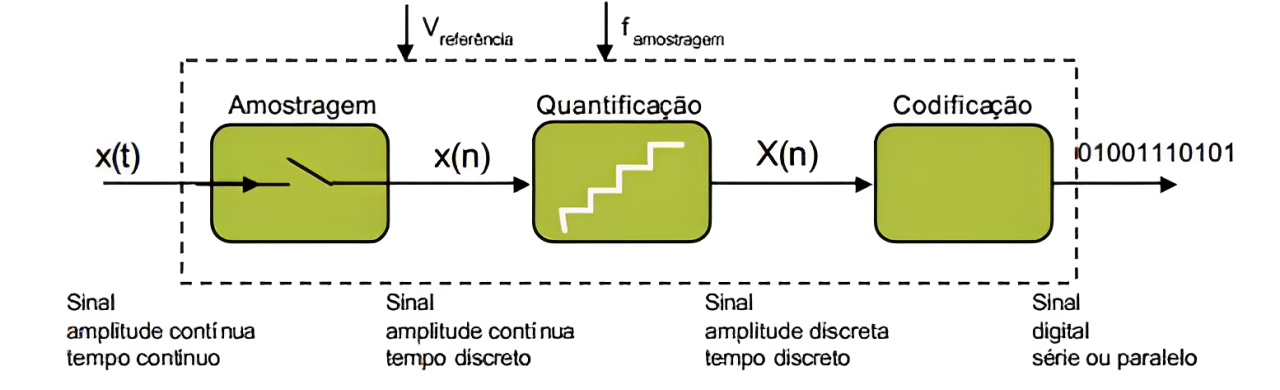
\includegraphics[width=1\linewidth]{conversorAD.png}
    \caption{Diagrama de blocos de conversor A/D}
    \label{fig:diagrama-conversor}
\end{figure}

Ao longo das décadas de estudo sobre conversores A/D, diversos modelos com diferentes princípios de funcionamento foram desenvolvidos. Entre os modelos disponíveis atualmente, destaca-se o conversor A/D de rampa dupla. Esse tipo de conversor, amplamente utilizado em multímetros digitais, apresenta vantagens significativas em relação a outros modelos, como o de rampa simples. Sua implementação é mais simples e oferece maior precisão, uma vez que elimina as variações causadas por resistores e capacitores no circuito.

O conversor A/D de Rampa Dupla é composto por elementos como resistores, capacitores, amplificadores operacionais e circuitos de controle, que atuam em conjunto para realizar a conversão do sinal analógico em digital com alta precisão. Esses componentes são organizados de forma a assegurar o funcionamento adequado das etapas de integração e desintegração do sinal. A configuração básica do conversor está ilustrada na Figura ~\ref{fig:basic_dual_slope_schematic}.

\begin{figure}[H]
    \centering
    \includesvg[width=1\linewidth]{03_results/assets/dual_slop_adc_basic_schematic.svg}
    \caption{Esquemático base do conversor ADC Rampa Dupla}
    \label{fig:basic_dual_slope_schematic}
\end{figure}

\subsection{Funcionamento do ADC de Rampa Dupla e Derivação Matemática}
O conversor ADC de Rampa Dupla opera em dois períodos de integração:

\subsubsection{Primeira Integração ($T_1$)}
Durante o período $T_1$, a chave conecta o sinal de entrada $V_I$ ao integrador. O integrador acumula a área do sinal de entrada, resultando em uma tensão $V_{CO}$ ao final de $T_1$. A duração de $T_1$ é fixa e depende da frequência do clock ($f_{clock}$) e da resolução ($N$) do conversor:
$$
    T_1 = \frac{2^N}{f_{clock}},
$$

A saída do integrador ao final de $T_1$ é dada por:
$$
    V_{CO} = -\frac{1}{R \cdot C} \int_0^{T_1} V_I \, dt = -\frac{V_I \cdot T_1}{R \cdot C}.
$$


\subsubsection{Segunda Integração ($T_2$)}
Após $T_1$, a chave conecta a tensão de referência negativa $-V_R$ ao integrador. Durante esse período, o integrador descarrega completamente, resultando em $V_{CO} = 0$ no final do tempo $T_2$. A tensão do integrador durante $T_2$ é descrita por:
\begin{align} \
    V_{CO} = -\frac{1}{R \cdot C} \left(\int_{T_1}^{T_1 + T_2} (-V_R) \, dt \right) - \frac{V_I \cdot T_1}{R \cdot C} \\
    V_{CO} = \frac{V_R \cdot T_2}{R \cdot C} - \frac{V_I \cdot T_1}{R \cdot C}.
\end{align}

Quando o capacitor descarrega completamente ($V_{CO} = 0$), temos:
$$
    \frac{V_R \cdot T_2}{R \cdot C} = \frac{V_I \cdot T_1}{R \cdot C}.
$$

Simplificando:
$$
    V_I \cdot T_1 = V_R \cdot T_2 \quad \Rightarrow \quad V_I = \frac{V_R \cdot T_2}{T_1}.
$$

\subsubsection{Relacionando o Tempo $T_2$ ao Valor Digital}
Sabendo que $T_1$ é fixo e equivale a $2^N / f_{clock}$, e que o tempo $T_2$ é proporcional ao valor digital $D$ gerado pelo contador, podemos reescrever $T_2$ como:
$$
    T_2 = D \cdot T_{clock}\, \text{, onde}\, T_{clock} = 1 / f_{clock}
$$

Substituindo $T_2$ na equação de $V_I$, temos:
$$
    V_I = V_R \cdot \frac{D \cdot T_{clock}}{T_1}.
$$

Substituindo $T_1 = 2^N / f_{clock}$:
$$
    V_I = V_R \cdot \frac{D \cdot (1 / f_{clock})}{2^N / f_{clock}} = V_R \cdot \frac{D}{2^N}.
$$

Assim, o valor digital $D$ que representa o sinal de entrada $V_I$ é dado por:
$$
    D = \frac{2^N \cdot V_I}{V_R}.
$$

Graficamente, o período de integração e desintegração de um conversor AD rampa dupla é representado pela figura \ref{fig:dual_slope_integrator_graph}, onde o período $T_{1}$ é a integração, quando o circuito integrador tem como entrada a tensão $V_{in}$ a ser convertida, e o período $T_{2}$ é a desintegração, que possui como entrada a tensão $V_{ref}$ de referência, que é fixa nas definições do projeto.
\begin{figure}
    \centering
    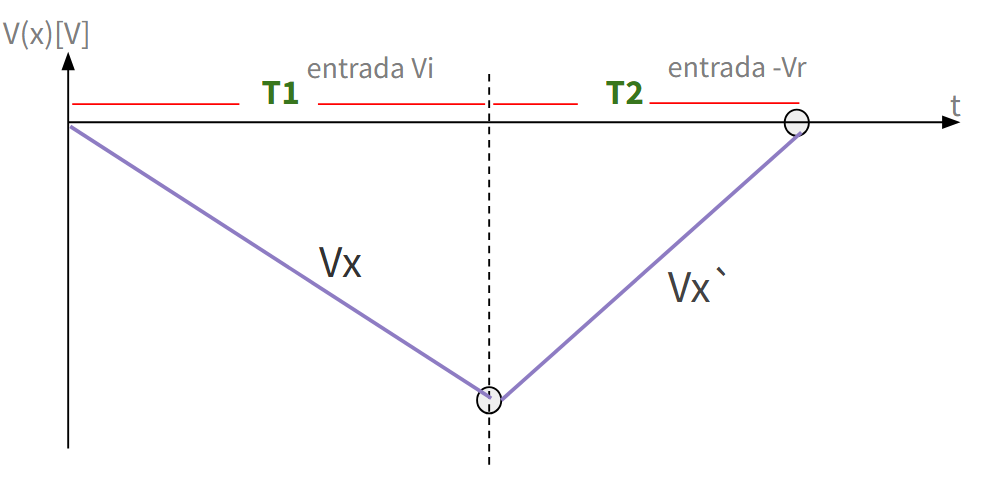
\includegraphics[width=1\linewidth]{dual_slope.png}
    \caption{Gráfico de saída do circuito integrador de um conversor rampa dupla}
    \label{fig:dual_slope_integrator_graph}
\end{figure}


\section{Resultados e discussões}
Para realizar o desenvolvimento do circuito, foi utilizado o simulador \textit{Falstad} (disponível em: \href{https://www.falstad.com/circuit/circuitjs.html}{falstad.com/circuit/circuitjs.html}). Como pode ser observado na Figura ~\ref{fig:circuit_svg}, foi simulado um circuito para a conversão de sinais de $1\, \text{Hz}$ de entrada alternada, com $5\, \text{Vpp}$.


\begin{figure}[H]
    \centering
    \resizebox{1\linewidth}{!}{%
        \includesvg{03_results/assets/circuit-20241128-2341.svg}
    }
    \caption{Diagrama do circuito de conversor analógico-digital Rampa Dupla}
    \label{fig:circuit_svg}
\end{figure}

Na etapa de construção do circuito, foram utilizados um resistor de $10\, \text{k} \Omega$ e um capacitor de $1\, \text{nF}$ no estágio integrador do conversor.

No desenvolvimento do conversor analógico-digital por Rampa Dupla, um aspecto essencial a considerar é a relação entre a frequência do sinal de entrada, a quantidade de níveis de quantização e o clock utilizado no contador. Para este projeto, determinamos inicialmente a quantidade de amostras que queremos ter em um período do sinal. Definimos esse valor em 250, ou seja, a cada 1/250 períodos da onda, o circuito realizará um ciclo completo de integração e desintegração. Com esse valor obtêm-se uma boa resolução sem um clock muito alto. Como nossa entrada é de $1\, \text{Hz}$, esse período é $1\,\text{s}$, então a cada $4\, \text{ms}$, teremos as duas rampas. O período de integração é de metade do período máximo de amostragem, $T_{1} = 2\, \text{ms}$.

Podemos verificar que um período de integração de $2\, \text{ms}$ resulta em um $T_{max} = 4\, \text{ms}$ utilizando a relação a seguir:

\begin{align*}
    T_{\text{max}}  & = T1 + T_{2\text{max}}                                          \\
    T_{2\text{max}} & = T1                                                            \\
    T_{\text{max}}  & = 2^{N} \times T_{\text{clock}} + 2^{N} \times T_{\text{clock}} \\
    T_{\text{max}}  & = 2 \times 2^{N} \times T_{\text{clock}}                        \\
    T_{\text{max}}  & = 2^{6+1} \times 0.00003125                                     \\
    T_{\text{max}}  & = 4 \text{ ms}
\end{align*}


A partir dessas definições, definimos o clock que será utilizado no contador para a obtenção do tempo de integração desejado de $2\, \text{ms}$:

\begin{align} \
    T_{1} = \frac{2^N}{f_{clock}} \\
    T_{1} = 2^N \cdot T_{clock}
\end{align}

onde:
\begin{enumerate}
    \item $T_1$ é o tempo total de integração ($2\, \text{ms}$)
    \item $2^N$ é o número de níveis de quantização (relacionado ao número de bits do conversor, $N$),
    \item $T_{clock}$ é o período do sinal de clock.
\end{enumerate}

Rearranjando a fórmula para encontrar $T_{clock}$, temos:

\begin{align} \
    T_{clock} = \frac{T_{1}}{2^N}               \\
    \text{Adotando} \, N=6 \, \text{bits:} \,
    T_{clock} = \frac{2 \times 10^{-3}}{64}     \\
    T_{clock} = 31.25 \times 10^{-6}\, \text{s} \\
    T_{clock} = 31.25\, \mu\text{s}
\end{align}

Assim, a frequência do clock ($f_{clock}$) é o inverso do período:

\begin{align} \
    f_{clock} = \frac{1}{T_{clock}}            \\
    f_{clock} = \frac{1}{31.25 \times 10^{-6}} \\
    \therefore f_{clock} \approx 32\, \text{kHz}
\end{align}

Portanto, o circuito deve operar com uma frequência de clock de $32\, \text{kHz}$ para realizar o processo de conversão com $2\, \text{ms}$ de período de integração.


Assim temos uma quantidade mínima de $\frac{1\, \text{s}}{0.004\text{s}(2ms*2)\ }$ amostras por período do sinal de entrada, ou seja 250 amostras por período.

A partir da Figura ~\ref{fig:falstad_simulator_output}, é possível observar duas representações gráficas dos sinais envolvidos no funcionamento do conversor analógico-digital (ADC) de Rampa Dupla. Na imagem B, está representada a entrada analógica alternada, um sinal senoidal de $1\, \text{Hz}$ com amplitude de $5\, \text{Vpp}$, que é o dado a ser convertido. Já na imagem A, temos a saída do circuito integrador, e a saída digital correspondente, que apresenta o sinal já amostrado e quantizado pelo ADC.

\begin{figure}[H]
    \centering
    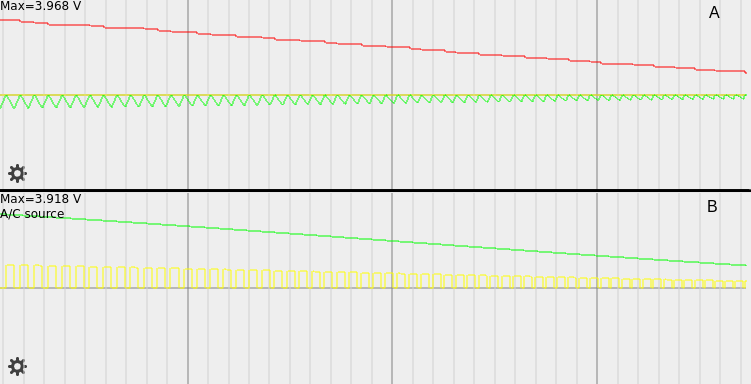
\includegraphics[width=1\linewidth]{03_results/assets/signal_output.png}
    \caption{A: Saída do ADC; B: Entrada A/C}
    \label{fig:falstad_simulator_output}
\end{figure}

O sinal quantizado e digitalizado, exibido na imagem A, reflete a discretização imposta pelo ADC. Cada degrau no gráfico representa um dos 64 níveis disponíveis no intervalo de operação, evidenciando o mapeamento do sinal senoidal contínuo em valores digitais. Nota-se que a resolução de 6 bits implica que a precisão do ADC depende tanto da estabilidade do clock quanto da qualidade do circuito integrador.

\subsection{Reduzindo para 25 amostras por período}
Caso a quantidade de amostras seja reduzida de 250 para 25 amostras por período do sinal de entrada, o período de amostragem aumenta proporcionalmente, passando de $4\,\text{ms}$ para $40\, \text{ms}$. Consequentemente, o tempo de integração ($T_1$) será de $20\, \text{ms}$, conforme definido anteriormente como metade do período de amostragem. A partir disso, podemos calcular a frequência de clock necessária.

Usando a mesma fórmula básica e adotando $N=6\,\text{bits}$, temos:
$$
    f_{clock} = \frac{2^N}{T_{1}} = \frac{64}{20 \times 10^{-3}} = 3.2 \, \text{kHz}
$$

Assim, ao reduzir a quantidade de amostras para 25, a frequência do clock também diminui para \textbf{$3.2 \, \text{kHz}$}. Essa alteração resulta em um menor consumo de energia e em um design menos exigente em termos de velocidade, ao custo de uma resolução temporal menor para o sinal de entrada.

Na Figura ~\ref{fig:falstad_simulator_output_25_samples}, observamos a saída do circuito operando com 25 amostras por período. Os principais pontos de inflexão do sinal ainda são capturados, mas há uma perda de detalhes na representação digital devido à menor densidade de amostras.

\begin{figure}[H]
    \centering
    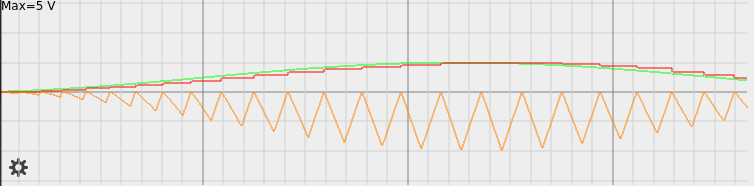
\includegraphics[width=1\linewidth]{03_results/assets/signal_output_25_samplings.png}
    \caption{Entrada A/C(verde), Saída Integrador (laranja), Saída Digital (vermelho)}
    \label{fig:falstad_simulator_output_25_samples}
\end{figure}

A perda de detalhes se dá devido à menor capacidade do ADC de acompanhar as rápidas variações do sinal de entrada. Em caso de sinais mais complexos ou de maior frequência, pode haver a introdução de maiores erros na representação digital do sinal.


\section{Conclusões}
Neste estudo, foi possível observar



\begin{thebibliography}{00}
    \bibitem{b1} SANCA, A.S. TEC430 - PROCESSAMENTO DIGITAL DE SINAIS : Notas de Aula. Universidade Estadual De Feira De Santana - Departamento De Tecnologia (DTEC). 2024.

    \bibitem{b2} Alan V. Oppenheim, Alan S. Willsky, and S. Hamid Nawab. Sinais e Sistemas. Prentice Hall, Sao Paulo, SP, Brasil, 3ª edição, 2012.

    \bibitem{proakis2006}
    Proakis, J. G., \& Manolakis, D. K. (2006). \textit{Digital Signal Processing: Principles, Algorithms, and Applications}. Pearson.

    \bibitem{cooley1965}
    Cooley, J. W., \& Tukey, J. W. (1965). An algorithm for the machine calculation of complex Fourier series. \textit{Mathematics of Computation}, 19(90), 297-301.

    \bibitem{lyons2010}
    Lyons, R. G. (2010). \textit{Understanding Digital Signal Processing}. Pearson.

    \bibitem{b3} L W. Couch. Digital and Analog Communication Systems. Prentice Hall, University of Florida (Electrical and Computer Engineering), New Jersey, 2ª edição, 2007.
\end{thebibliography}


\appendix
\section{Detalhes Adicionais}
\subsubsection{Frequência de Amostragem: 5 kHz}

Nesta seção, analisamos o comportamento de um sinal senoidal de 1 kHz com uma frequência de amostragem configurada para 5 kHz. Com essa taxa, coletamos um total de 200 amostras, permitindo observar o sinal no domínio do tempo e seu espectro de frequência.

\begin{figure}[H]
    \centering
    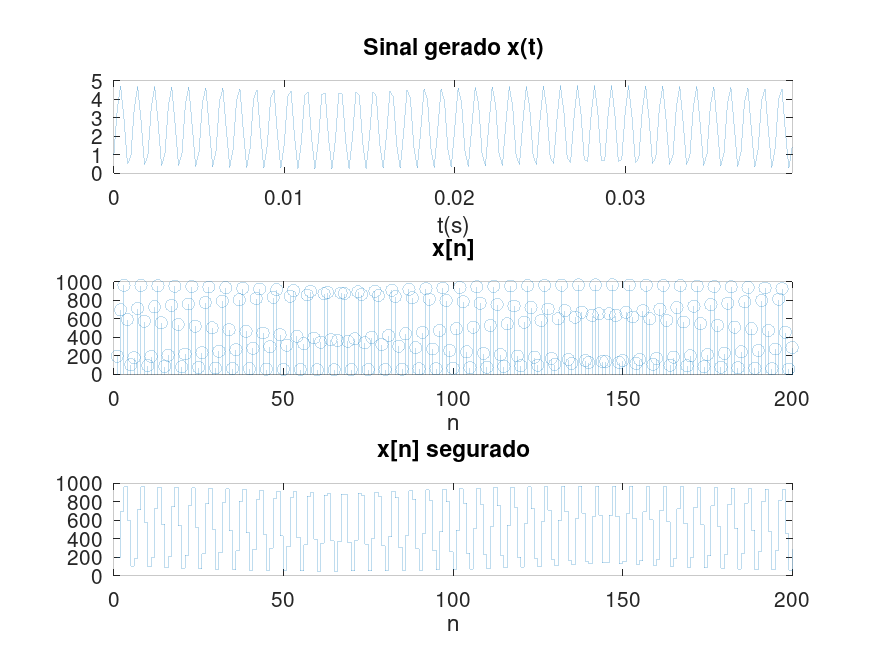
\includegraphics[width=1\linewidth]{03_results/assets/sin__1KHz_fs5k_SIGNAL_200smp.png}
    \caption{Sinal senoidal de 1 kHz com frequência de amostragem de 5 kHz, exibindo 200 amostras no domínio do tempo.}
    \label{fig:signal-5kHz-1kHz-200smp}
\end{figure}

\begin{figure}[H]
    \centering
    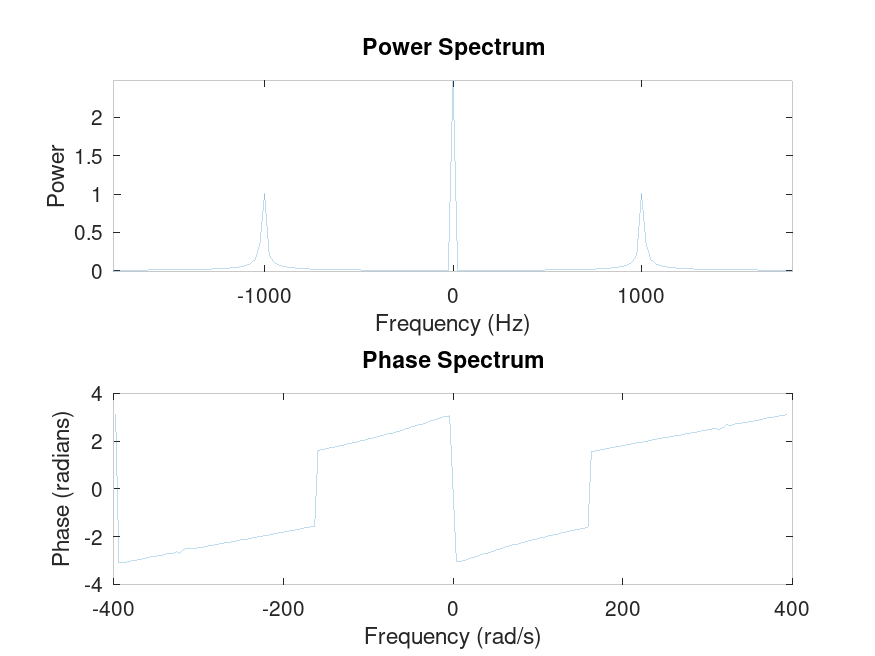
\includegraphics[width=1\linewidth]{03_results/assets/sin__1KHz_fs5k_SPECTRUM_200smp.png}
    \caption{Espectro do sinal senoidal de 1 kHz, amostrado a 5 kHz, com 200 amostras.}
    \label{fig:spectrum-5kHz-1kHz-200smp}
\end{figure}

\subsubsection{Frequência de Amostragem: 10 kHz}

Aqui, o sinal senoidal de 1 kHz foi amostrado a uma frequência de 10 kHz, permitindo uma coleta mais densa de pontos no domínio do tempo, totalizando 400 amostras.

\begin{figure}[H]
    \centering
    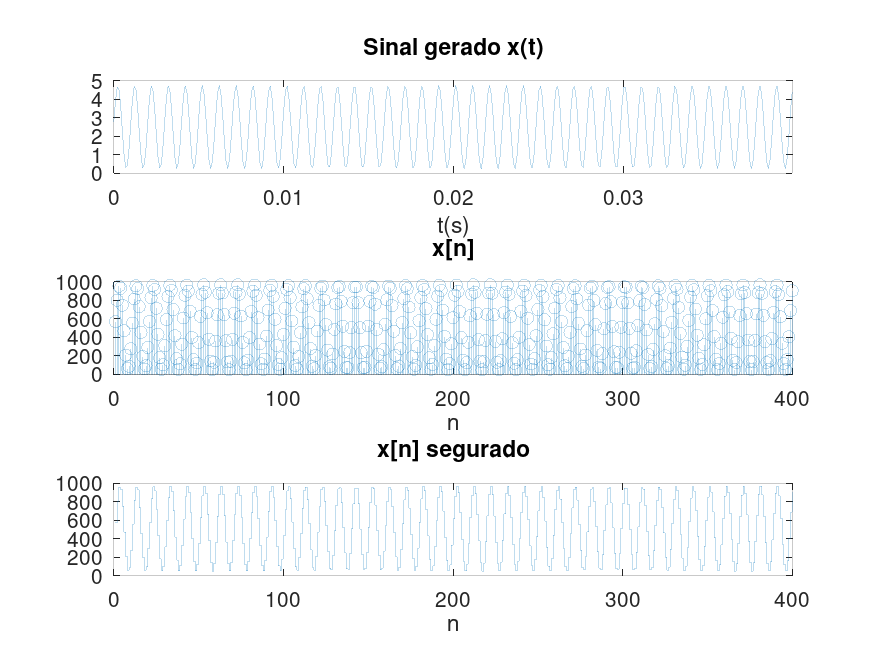
\includegraphics[width=1\linewidth]{03_results/assets/sin__1KHz_fs10k_SIGNAL_400smp.png}
    \caption{Sinal senoidal de 1 kHz amostrado a 10 kHz, apresentando 400 amostras no domínio do tempo.}
    \label{fig:signal-10kHz-1kHz-400smp}
\end{figure}

\begin{figure}[H]
    \centering
    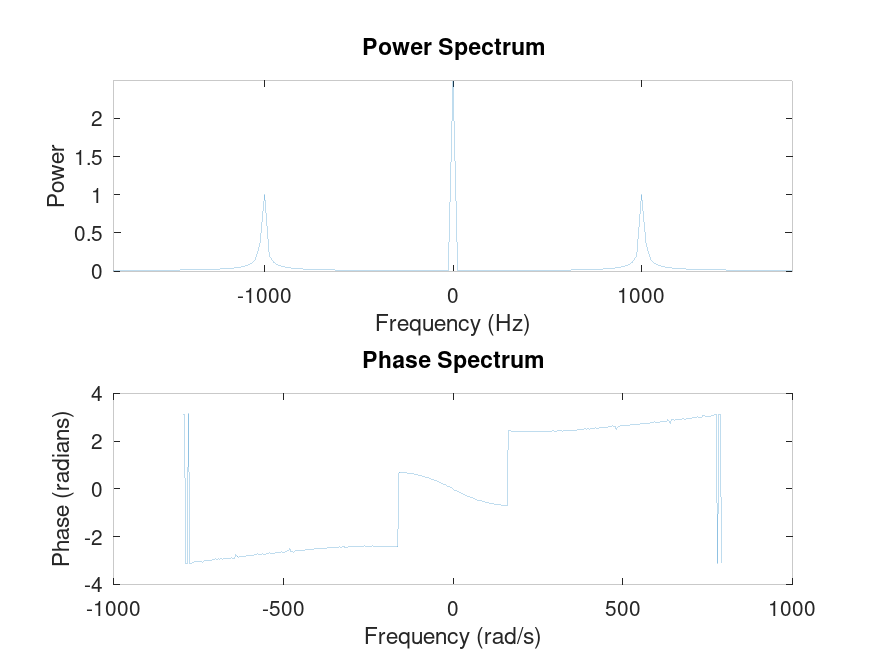
\includegraphics[width=1\linewidth]{03_results/assets/sin__1KHz_fs10k_SPECTRUM_400smp.png}
    \caption{Espectro do sinal senoidal de 1 kHz, com frequência de amostragem de 10 kHz e 400 amostras.}
    \label{fig:spectrum-10kHz-1kHz-400smp}
\end{figure}

\subsubsection{Frequência de Amostragem: 20 kHz}

Nesta seção, o sinal senoidal de 10 kHz foi amostrado a uma taxa de 20 kHz. Com essa configuração, coletamos 600 amostras, o que permite observar detalhadamente as características temporais e espectrais do sinal.

\begin{figure}[H]
    \centering
    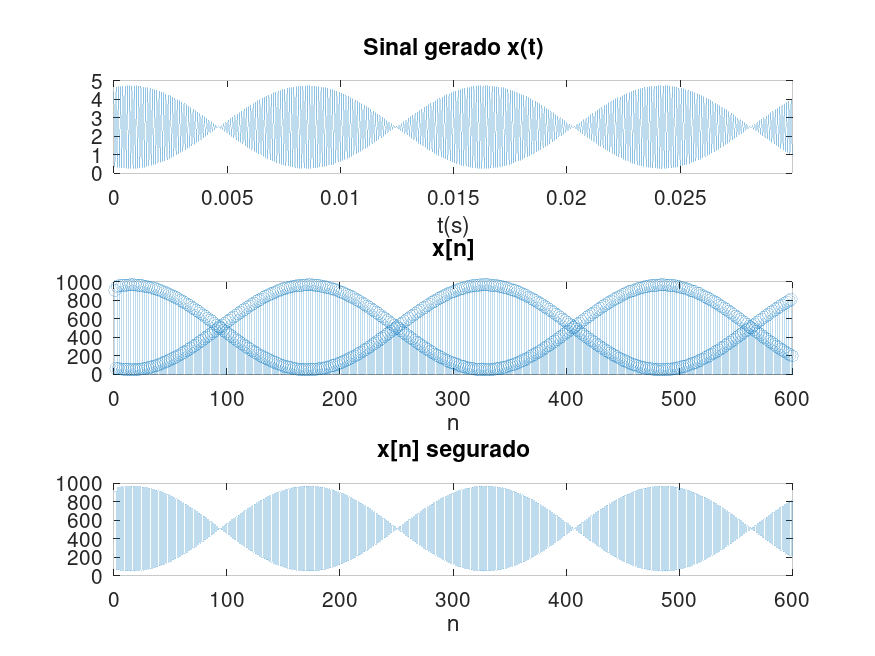
\includegraphics[width=1\linewidth]{03_results/assets/sin__10KHz_fs20k_SIGNAL_600smp.png}
    \caption{Sinal senoidal de 10 kHz com frequência de amostragem de 20 kHz, exibindo 600 amostras no domínio do tempo.}
    \label{fig:signal-20kHz-10kHz-600smp}
\end{figure}

\begin{figure}[H]
    \centering
    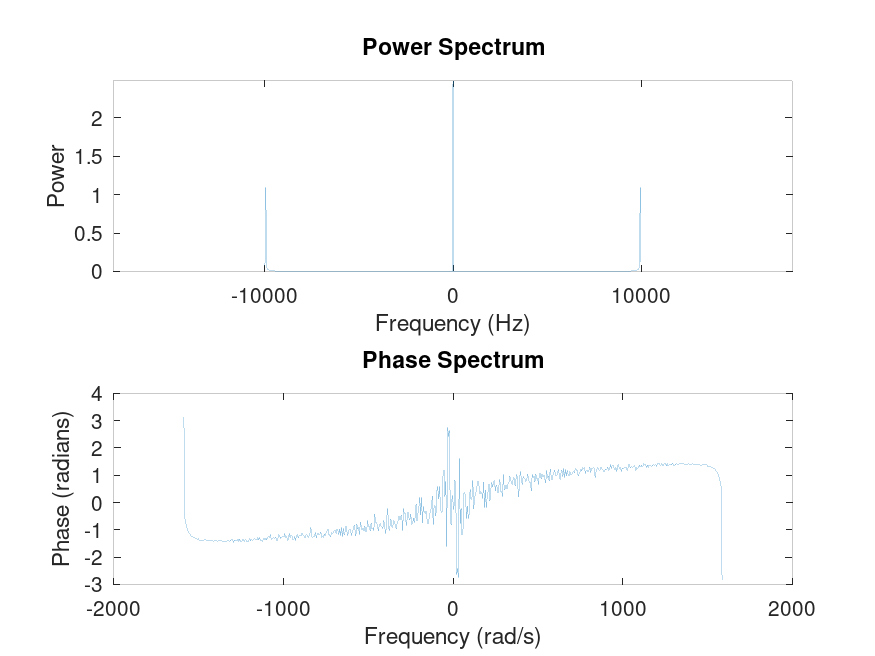
\includegraphics[width=1\linewidth]{03_results/assets/sin__10KHz_fs20k_SPECTRUM_600smp.png}
    \caption{Espectro do sinal senoidal de 10 kHz, amostrado a 20 kHz, com 600 amostras.}
    \label{fig:spectrum-20kHz-10kHz-600smp}
\end{figure}

\subsubsection{Frequência de Amostragem: 50 kHz}

Por fim, o sinal senoidal de 10 kHz foi amostrado a uma frequência de 50 kHz. Com essa configuração de alta resolução, obteve-se 600 amostras, permitindo uma análise detalhada no domínio do tempo e frequência.

\begin{figure}[H]
    \centering
    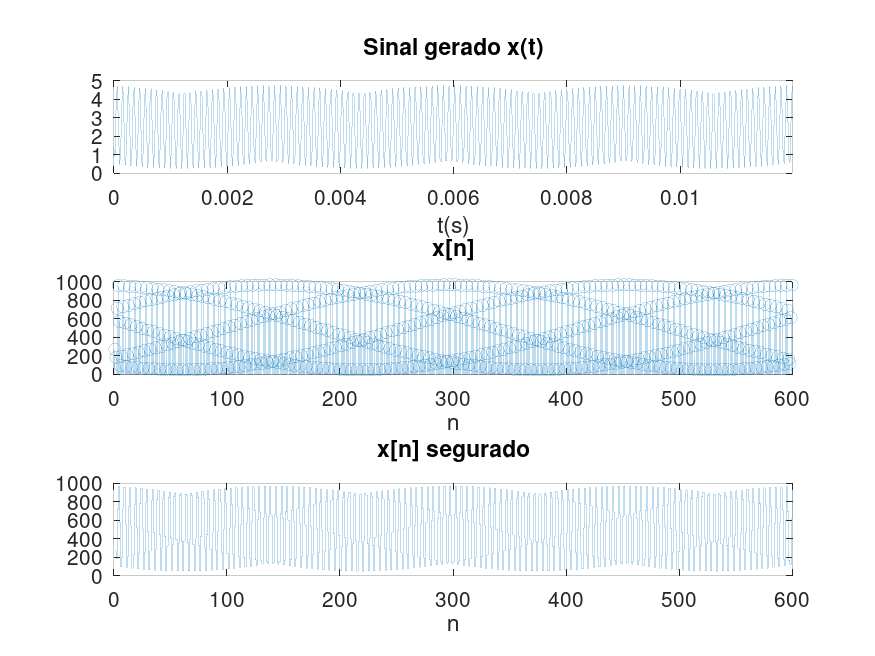
\includegraphics[width=1\linewidth]{03_results/assets/sin__10KHz_fs50k_SIGNAL_600smp.png}
    \caption{Sinal senoidal de 10 kHz com frequência de amostragem de 50 kHz, exibindo 600 amostras no domínio do tempo.}
    \label{fig:signal-50kHz-10kHz-600smp}
\end{figure}

\begin{figure}[H]
    \centering
    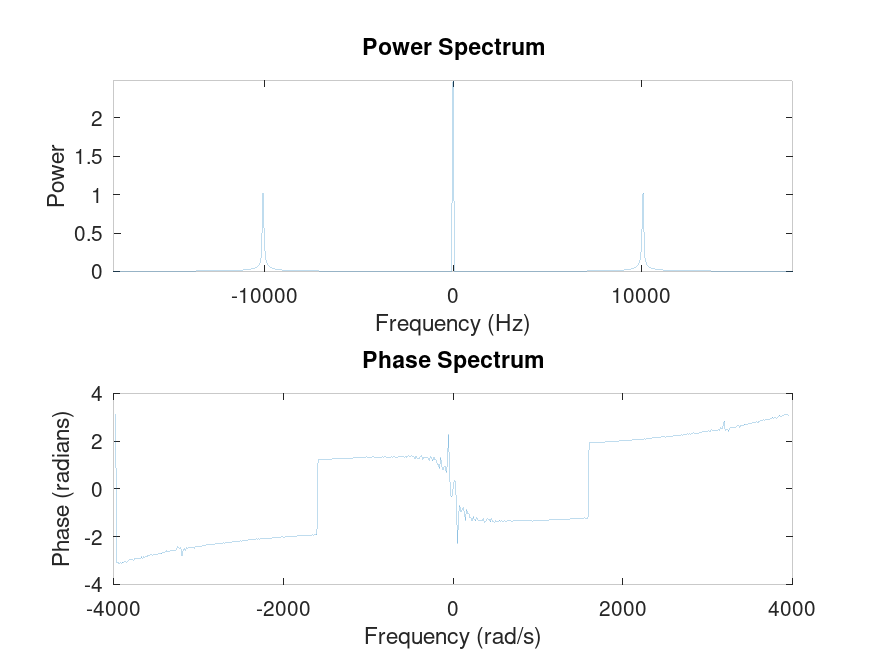
\includegraphics[width=1\linewidth]{03_results/assets/sin__10KHz_fs50k_SPECTRUM_600smp.png}
    \caption{Espectro do sinal senoidal de 10 kHz, amostrado a 50 kHz, com 600 amostras.}
    \label{fig:spectrum-50kHz-10kHz-600smp}
\end{figure}

\begin{itemize}
    \item Com o aumento da frequência de amostragem, o espectro do sinal representa com mais precisão a frequência original. Por exemplo, para um sinal de 1 kHz, uma amostragem de 5 kHz oferece resolução aceitável, mas com possíveis distorções no pico de frequência devido à menor densidade de amostras. Em frequências de amostragem mais altas, como 10 kHz ou 20 kHz, o espectro apresenta um pico mais claro e preciso, indicando menor quantização e menos aliasing.
    
    \item A quantidade de amostras também afeta a resolução espectral. Com 200 ou 400 pontos, o espectro apresenta picos mais largos e menos nítidos. Ao aumentar para 600 amostras, os picos de frequência ficam mais estreitos e definidos, pois o intervalo entre as frequências discretas diminui, proporcionando um espectro mais detalhado.
\end{itemize}


\end{document}
